\chapter{Basic Concepts of Deep Learning}

In recent years, artificial intelligence (AI) and deep learning (DL) have transformed the way we approach some of the most complex challenges in hydrology, geoscience, and environmental science. These technologies have moved beyond simple predictions to achieve groundbreaking feats, such as NASA’s DL-based models for real-time global precipitation estimates and large-scale climate simulations that capture fine-grained details of weather extremes. Researchers have even developed AI-driven systems akin to generative pre-trained transformer (GPT), trained on decades of environmental data, to assist in forecasting water resource availability and identifying critical climate trends.

The promise of AI and DL in water sciences is immense. From reimagining flood preparedness with hyper-accurate early warning systems to unraveling the mysteries of groundwater depletion with global-scale models, the potential applications are as vast as they are impactful. At the same time, this field is highly competitive, with scientists racing to harness these tools to address urgent environmental issues, inform policy decisions, and secure a sustainable future.

This chapter introduces the foundational ideas of AI and DL, exploring how these tools have already reshaped water and climate sciences and the transformative possibilities that lie ahead.

\begin{figure}[!h]
    \centering
    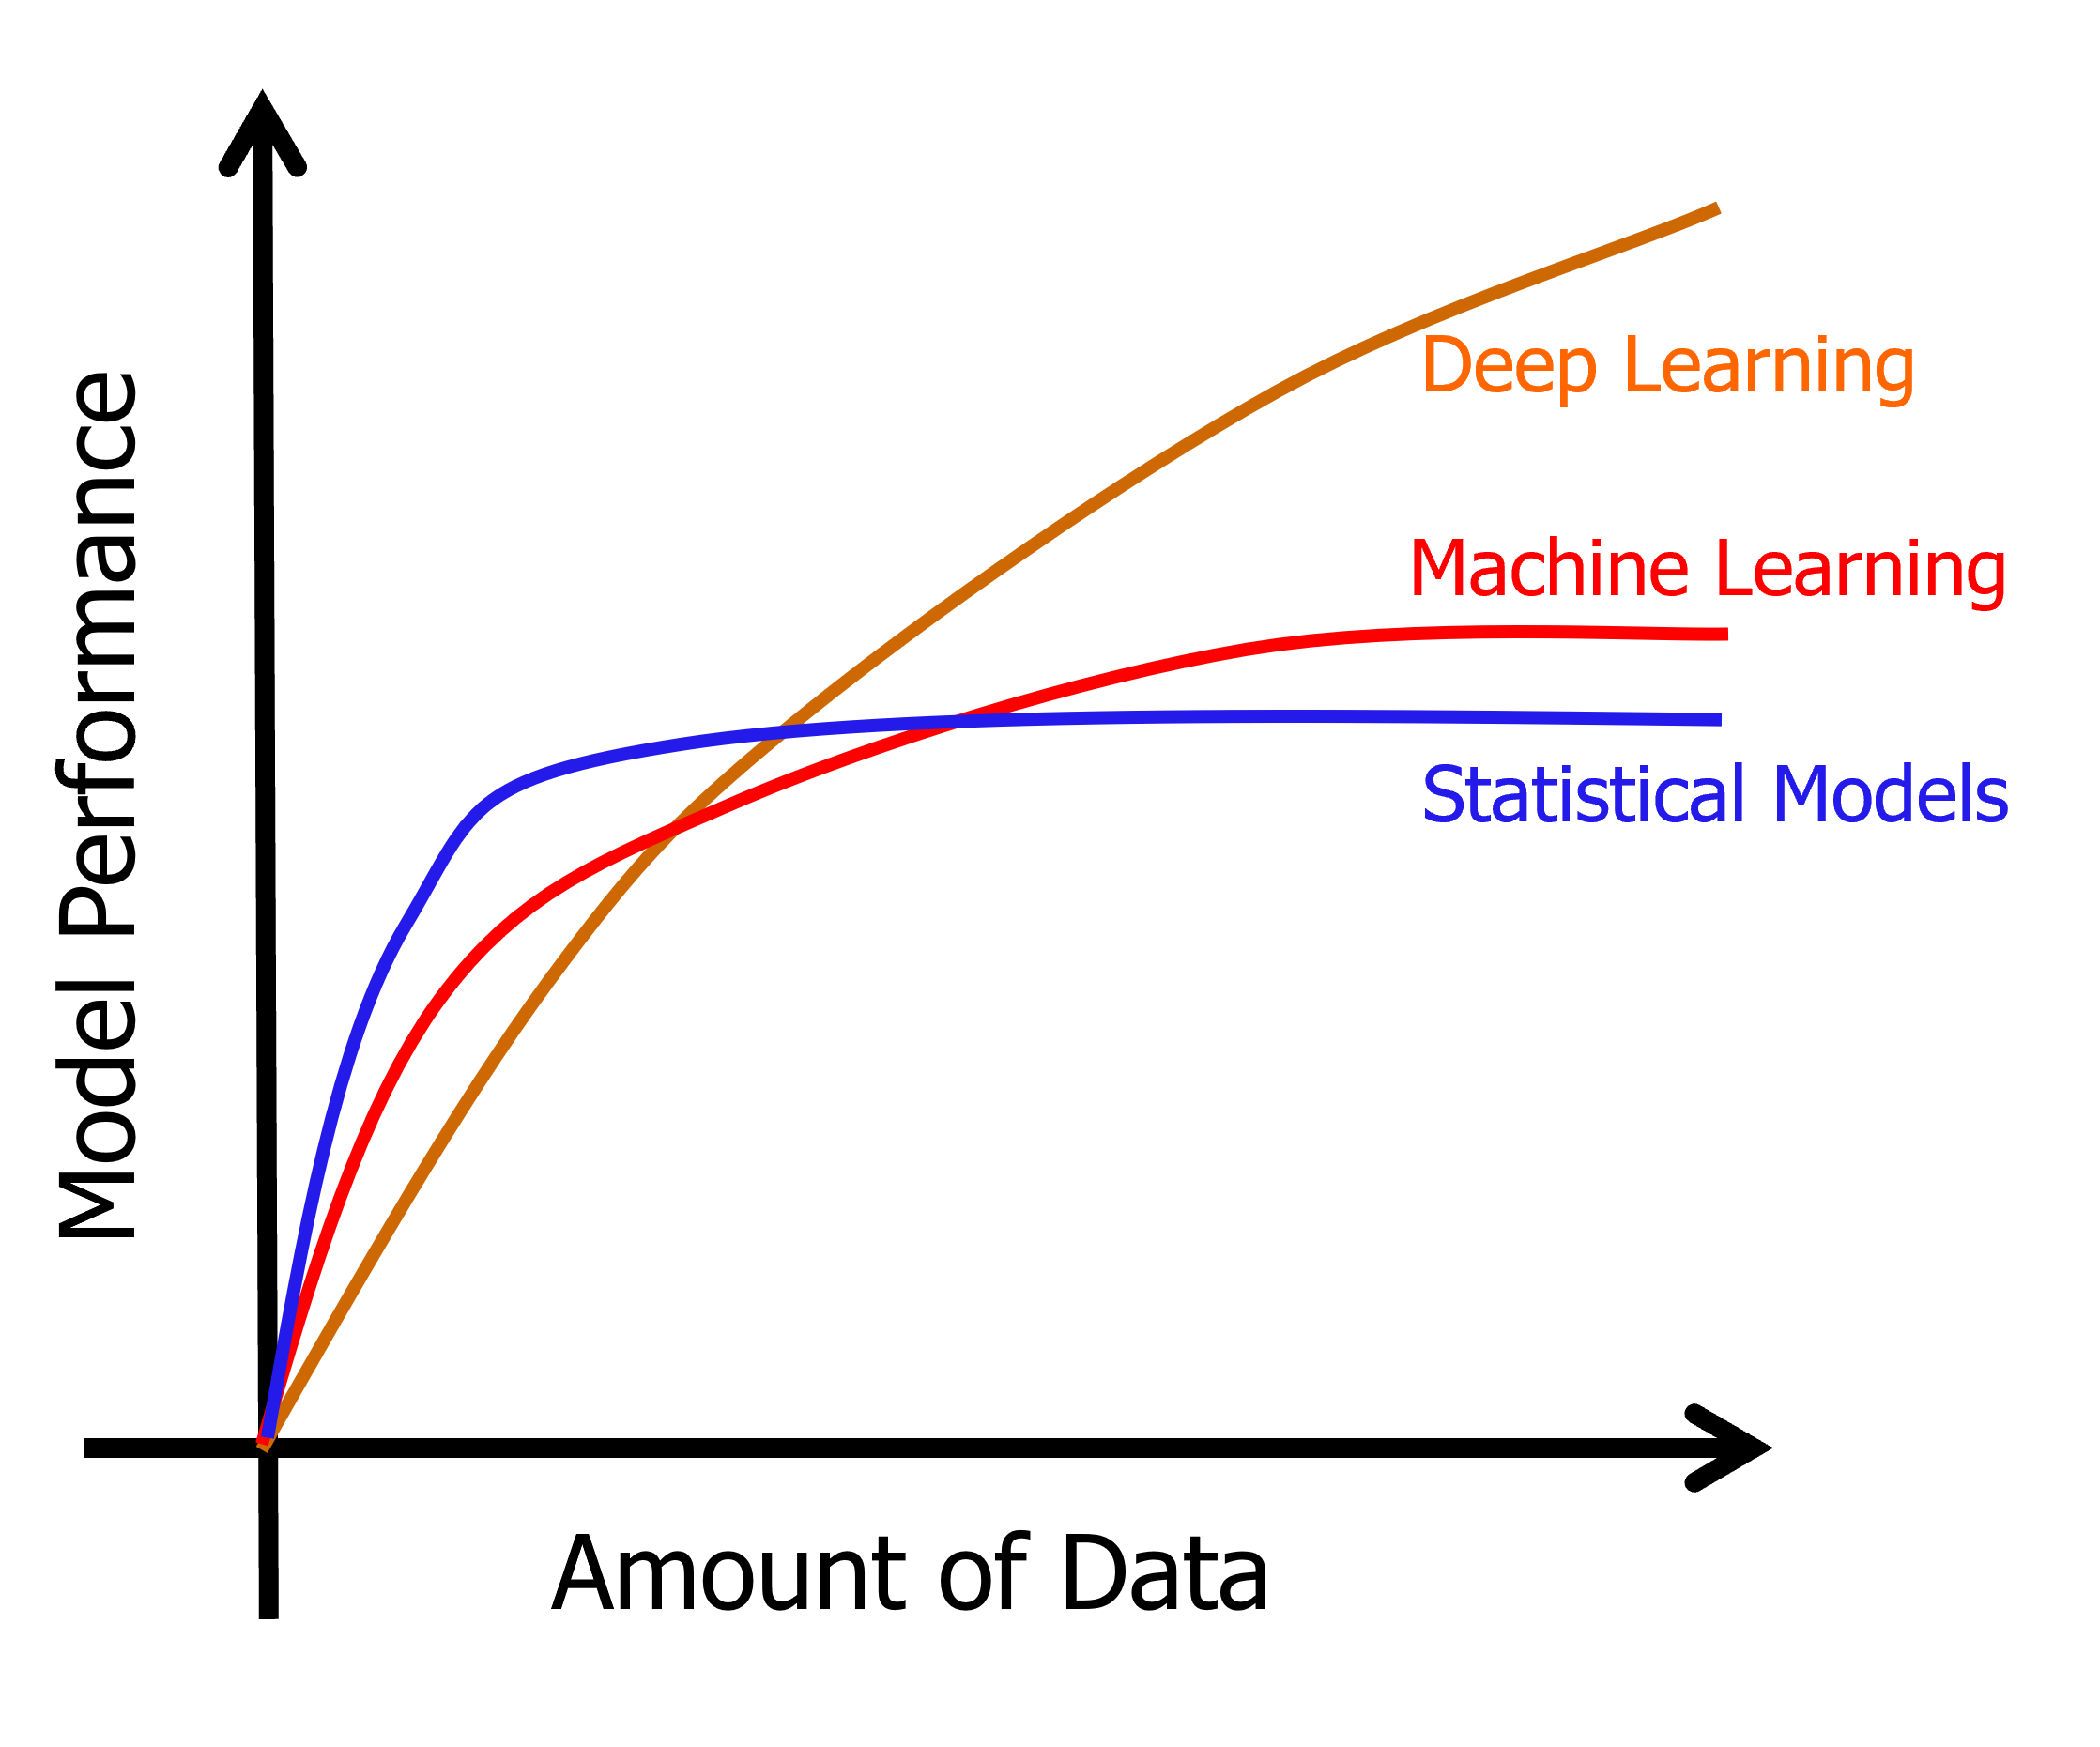
\includegraphics[width=1\linewidth]{images/What is DL.png}
    \caption{Comparison of model performance across increasing data availability for statistical models, machine learning, and deep learning}
    \label{fig:what_is_dl}
\end{figure}


\section{Understanding AI, ML, and DL: How They Relate to Each Other}
Before diving into deep learning and its applications, it’s essential to understand its roots and how it fits into the broader picture of AI and ML. Think of AI, ML, and DL as nested boxes, where each is a subset of the previous one.
\begin{figure}
    \centering
    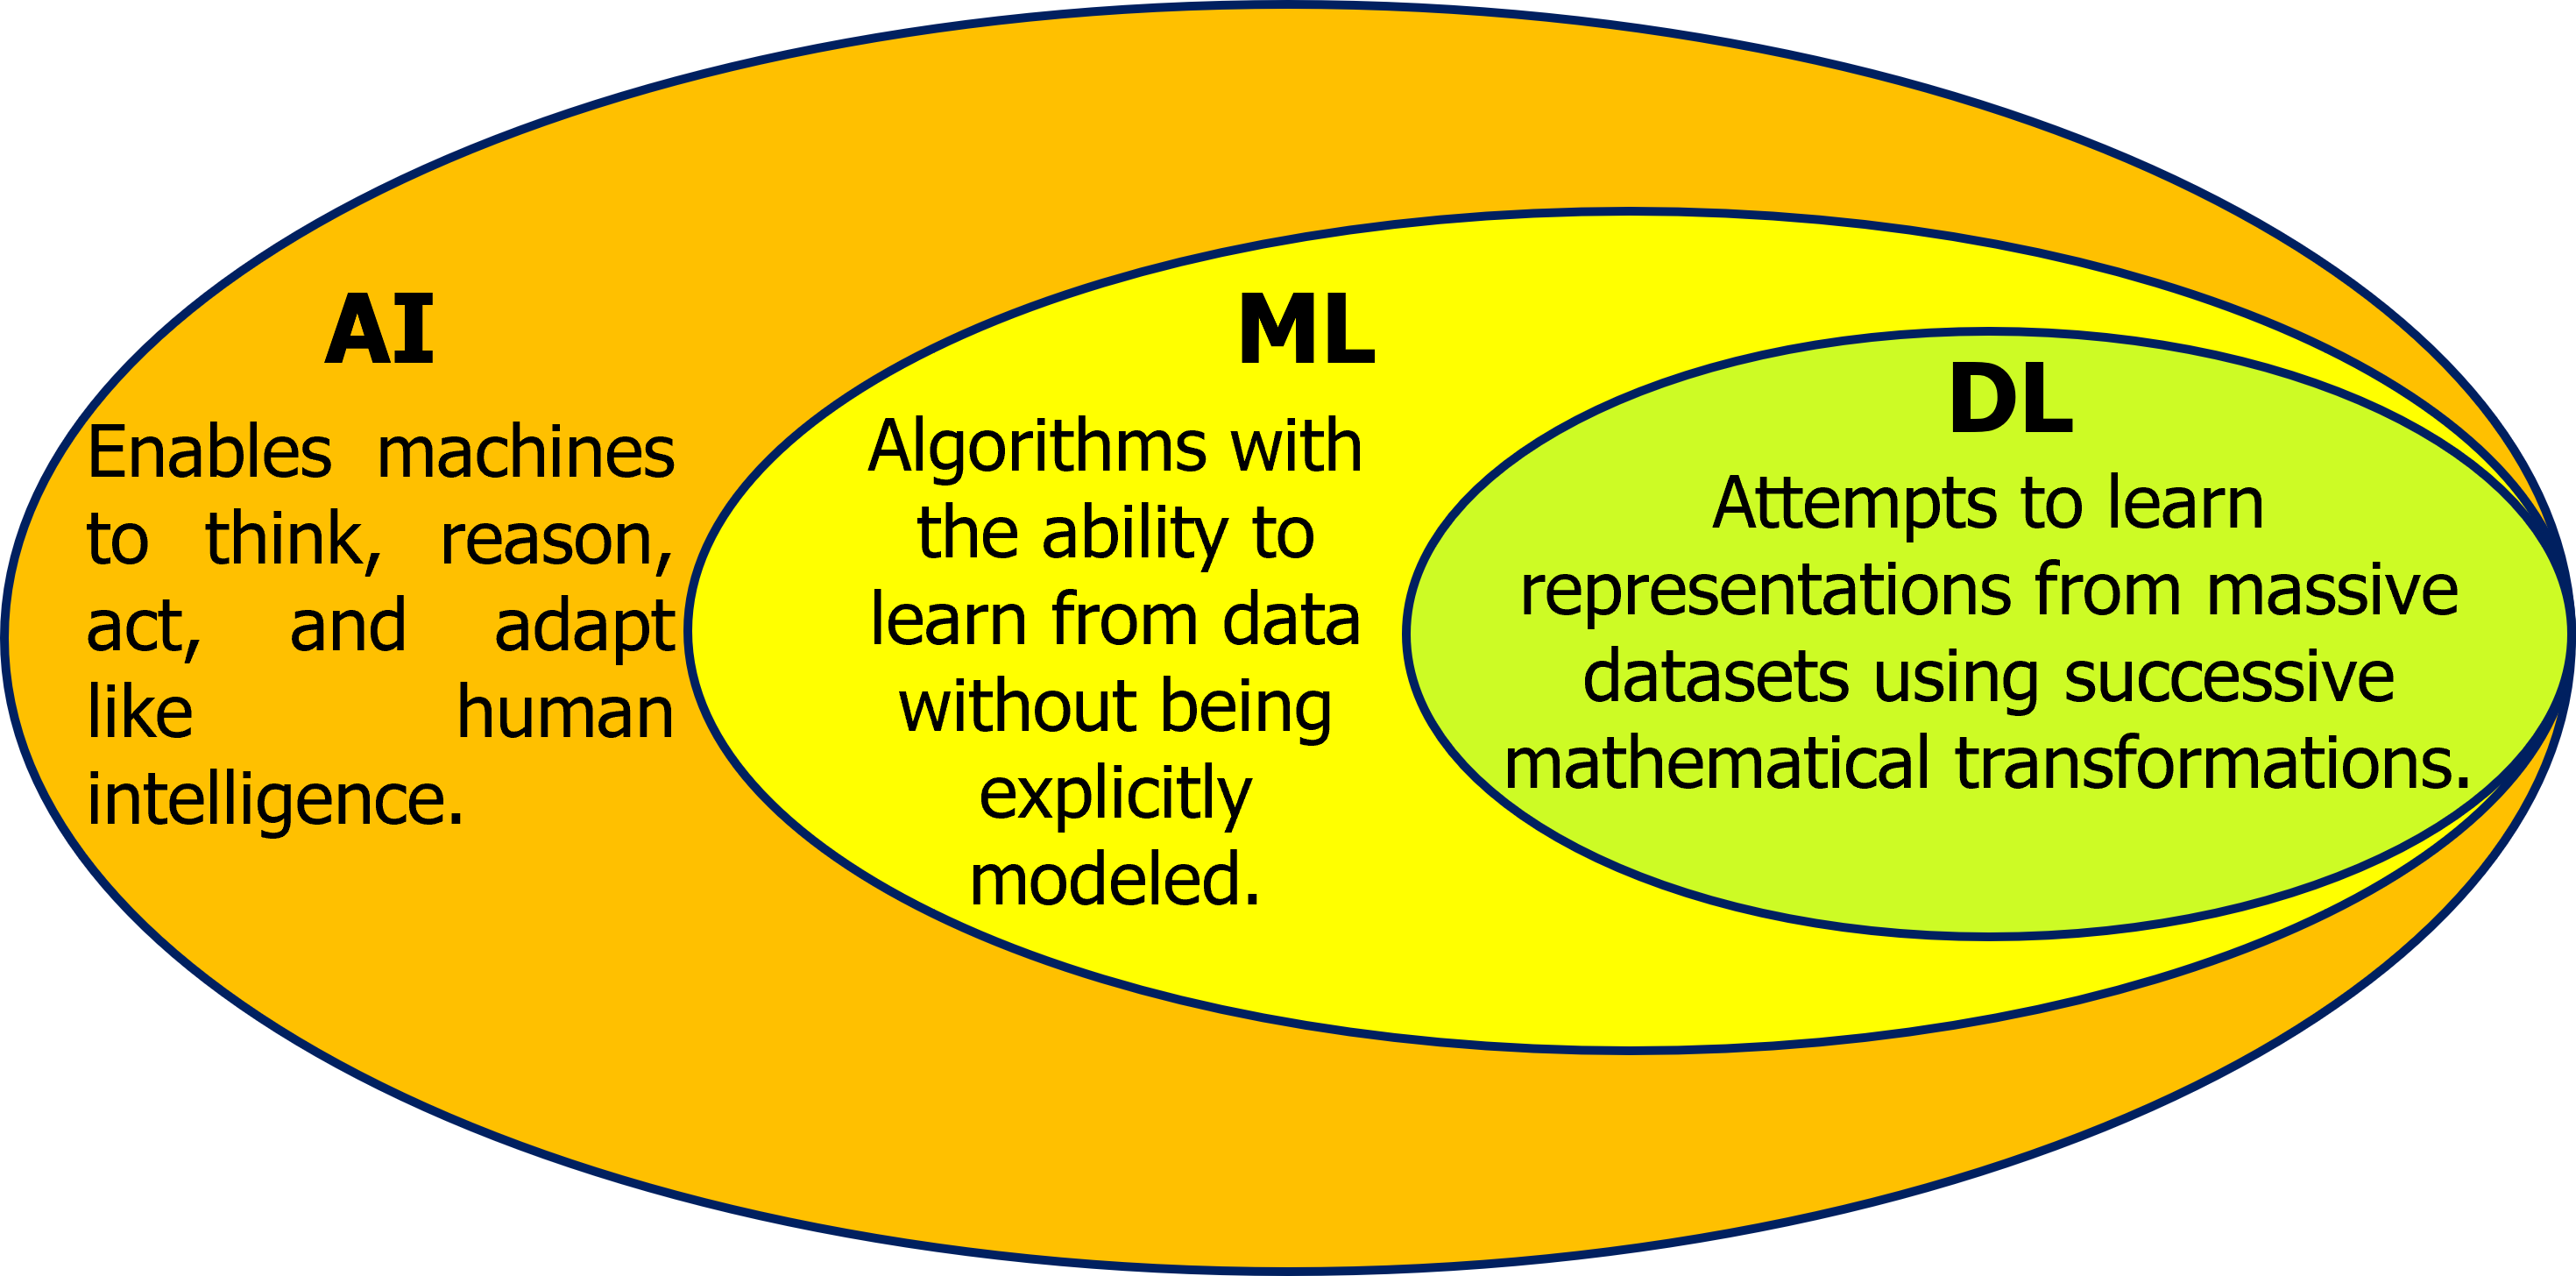
\includegraphics[width=0.99\linewidth]{images/ai-ml-dl.png}
    \caption{Illustrates the hierarchical relationship between Artificial Intelligence (AI), Machine Learning (ML), and Deep Learning (DL), with AI representing a broader field, ML as its subset, and DL as a subset of machine learning}
    \label{fig:ai-ml-dl}
\end{figure}
\subsection{Artificial Intelligence: The Big Picture}
The term Artificial Intelligence (AI) was coined in the mid-20th century, during a time when computers had only begun to show potential as tools capable of performing tasks resembling human intellect. AI broadly refers to systems designed to automate intellectual tasks typically performed by humans, such as reasoning, learning, and problem-solving.

In its earliest days, AI systems were built using hardcoded rules—a paradigm known as \textit{symbolic AI}. These systems were excellent at solving narrowly defined, logical problems, like playing chess or diagnosing straightforward faults in machinery. For example, early AI systems could be programmed to predict river discharge based on a fixed set of rules derived from historical data patterns. Another example could be simulating the operation of a water distribution network to optimize supply during drought conditions. These rule-based systems worked well for straightforward scenarios but struggled when faced with the complexity and variability of real-world problems, such as predicting extreme floods caused by unexpected climatic events.

The shortcomings of symbolic AI led to the realization that complex, fuzzy tasks—like understanding the nuances of water quality dynamics in a lake or recognizing patterns in satellite imagery of drought-stricken areas—could not be solved by explicitly defining every rule. This gave rise to new approaches like \textit{Machine Learning}, which relies on the computer learning from data rather than being explicitly programmed.

\subsection{Machine Learning(ML)}

ML emerged as a transformative step in AI's evolution. It addressed a key limitation of early AI systems, which relied on programmers explicitly defining rules for every possible situation. ML posed a new question: \textit{Could a machine learn the rules itself from data?}

This paradigm shift gave birth to a new programming approach. Instead of explicitly instructing machines, ML systems learn by example. Humans supply \textbf{input data} and the corresponding \textbf{desired outputs}, and the machine learns to infer the rules that map the inputs to the outputs. These learned rules can then be generalized to make predictions on new, unseen data. Classical programming operates as follows (see Figure \ref{fig:ml}):
\begin{enumerate}
    \item \textbf{Humans define rules} to process data.
    \item Machines apply these rules to produce outputs.
\end{enumerate}

Machine learning, on the contrary, inverts this process:
\begin{enumerate}
    \item Humans provide \textbf{ data samples and their outputs}.
    \item The machine generates the rules that connect the data to its output.
\end{enumerate}
\begin{figure}
    
    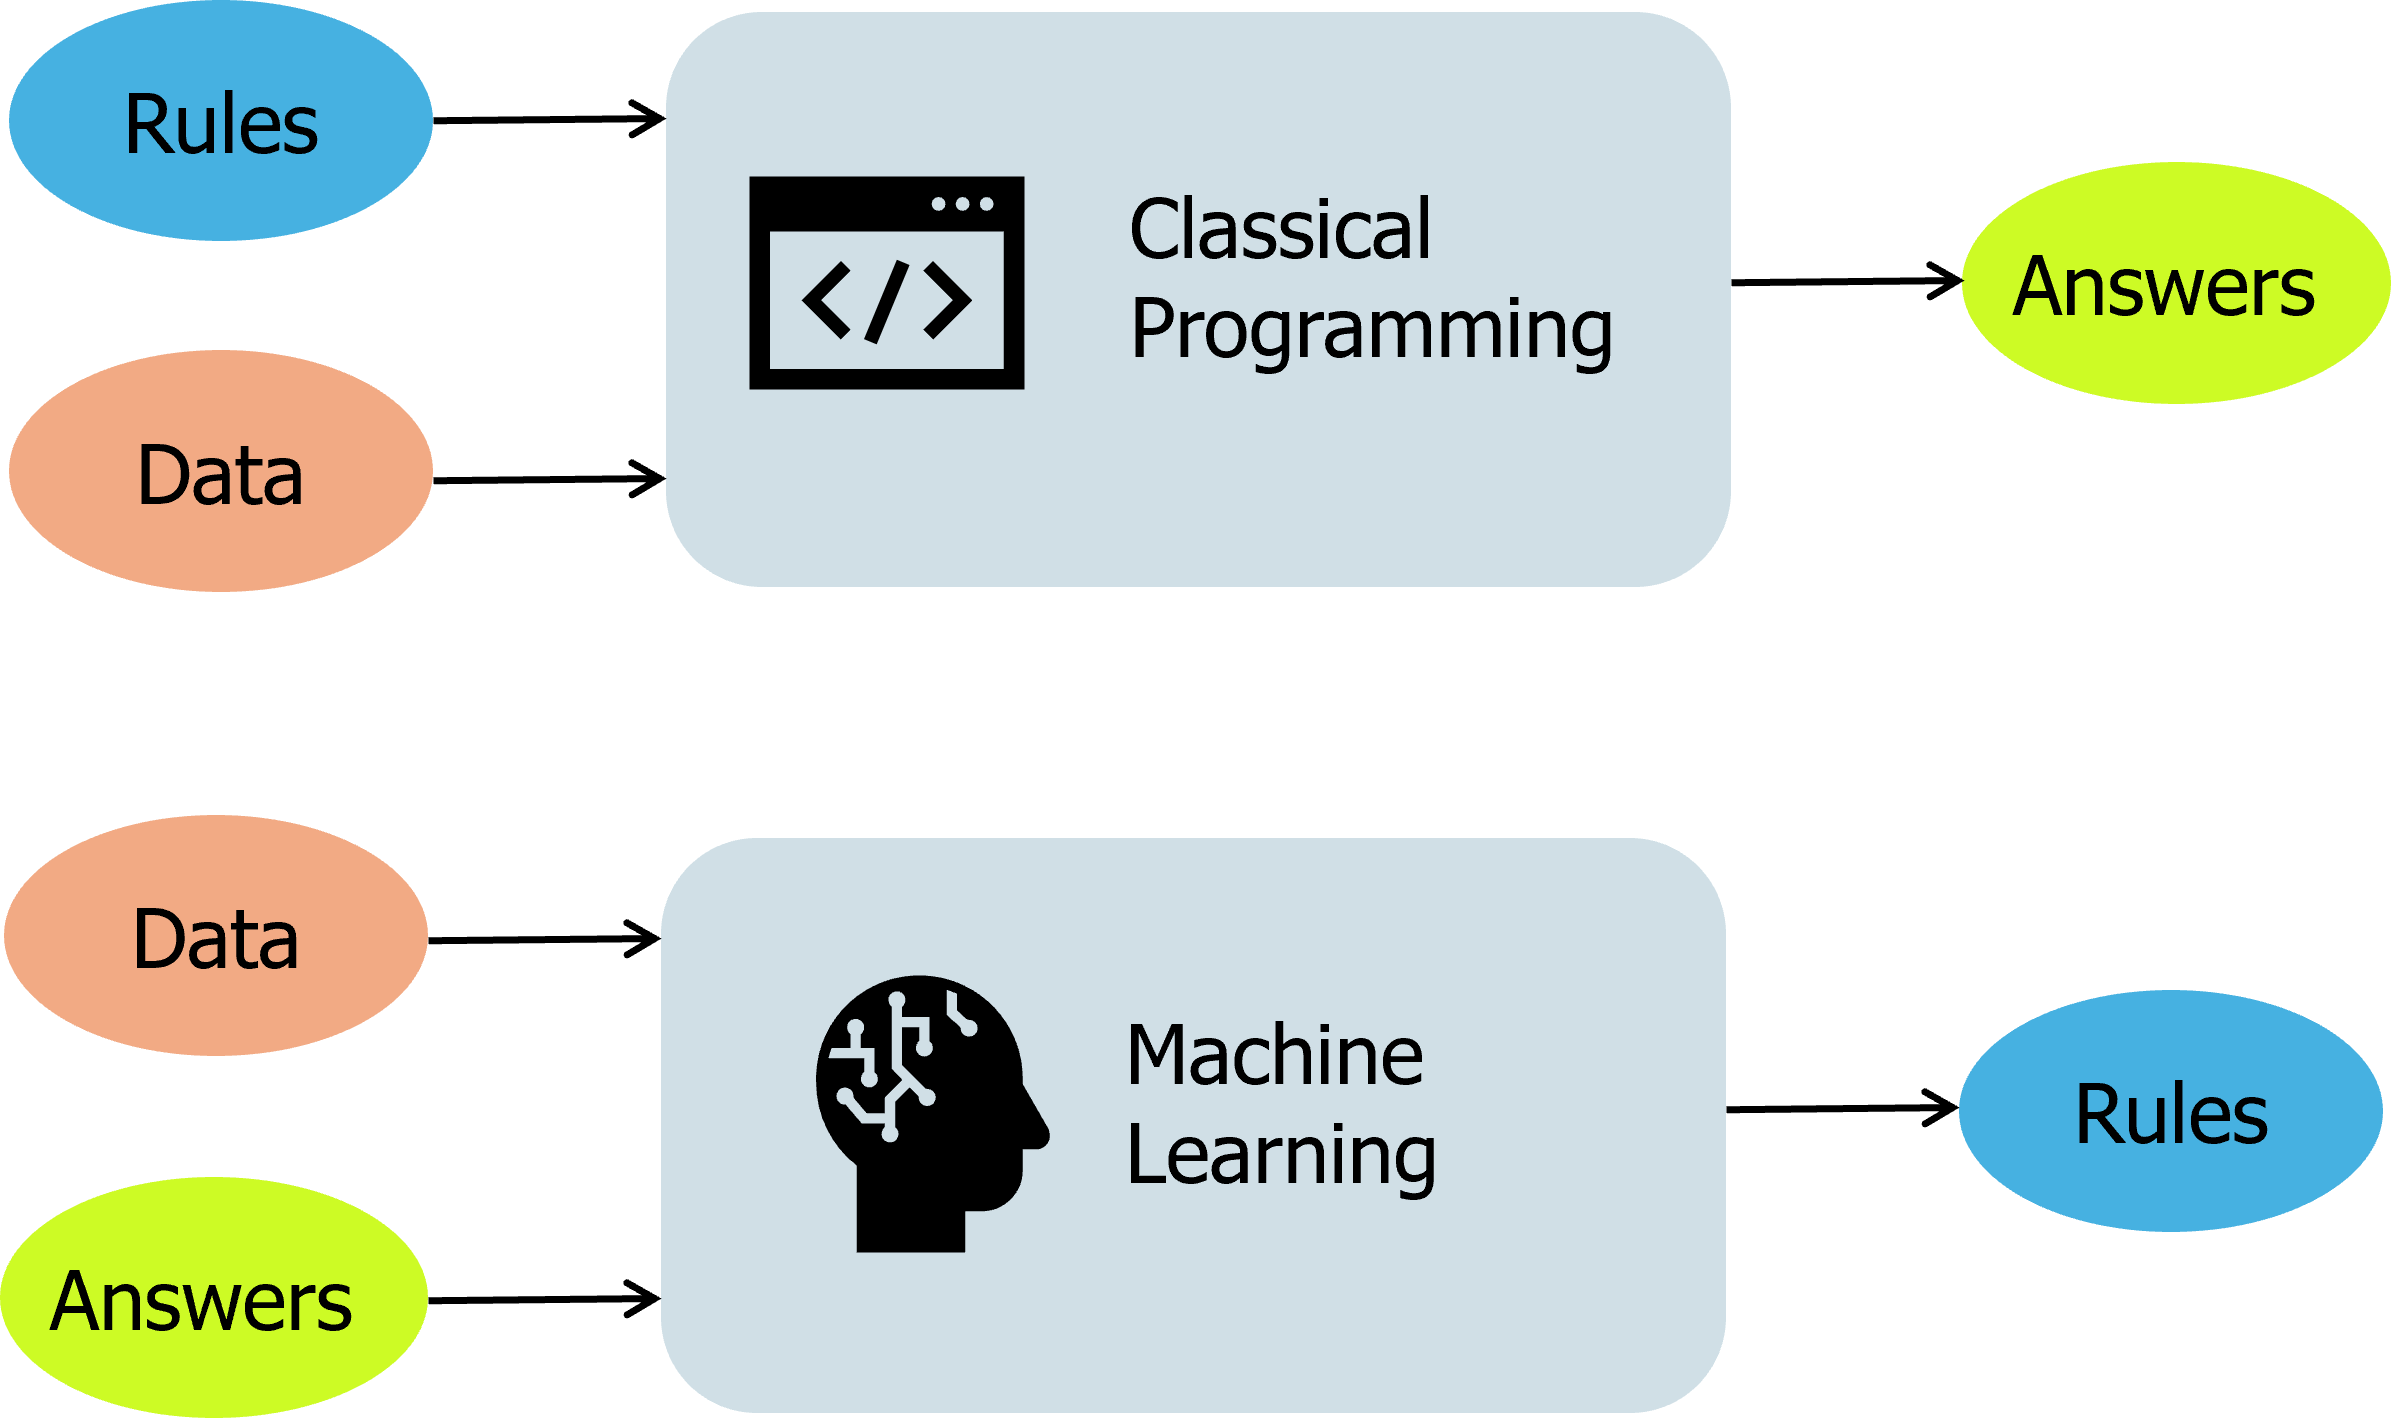
\includegraphics[width=0.75
    \linewidth]{images/ml.png}
    \caption{Classical programming vs Machine Learning (ML)}
    \label{fig:ml}
\end{figure}
This shift is similar to teaching a student by showing examples rather than lecturing about every concept. The result is a machine that can adapt and improve its performance without human intervention in the crafting of detailed instructions.

\subsubsection{Example from Hydrology}

To automate \textit{streamflow prediction}, classical programming might involve encoding complex hydrological models with explicit equations for runoff and infiltration. However, this approach struggles with unmodeled phenomena such as sudden changes in land use or climate variability.

With ML, the system is fed:
\begin{itemize}
    \item Historical data \textbf{ of rainfall and runoff} (input).
    \item Corresponding observed \textbf{streamflow values} (output).
\end{itemize}

The machine learns patterns and relationships within these data, creating a model capable of predicting stream flow under new rainfall scenarios without being explicitly programmed for every possible condition.

\subsection{Why ML Became So Popular in hydrology?}

Machine learning began to flourish in the 1990s especially in the computer vision domain, but The adoption of machine learning in hydrology accelerated around 2005 and surged post-2010 due to three key drivers
\begin{itemize}
    \item \textbf{Diverse and Large Datasets:}  The integration of multi-source, multi-scale, and high-dimensional datasets—ranging from remote sensing imagery to climate model outputs—enabled researchers to study nonlinear interactions across various hydrological processes. These datasets provide the foundation for ML to extract complex patterns and insights that traditional methods often miss.
    \item \textbf{Advances in Computational Power:}  The availability of high-performance GPUs, such as NVIDIA's latest models, revolutionized ML training. These GPUs enable the processing of vast hydrological datasets at high resolution, a task once deemed computationally prohibitive.
    \item \textbf{Handling Complexity: } Machine learning thrives on extracting actionable insights from complex, high-dimensional data. Unlike traditional statistics, which struggle with such datasets, ML excels in finding relationships and patterns that drive inference and prediction in hydrological systems.
    
\end{itemize}

ML has proven particularly powerful in tasks where patterns and predictions are required, such as:
\begin{itemize}
    \item \textit{Flood risk mapping from satellite imagery.}
    \item \textit{Estimating groundwater levels from precipitation and temperature data.}
\end{itemize}

Unlike traditional statistical methods, which rely heavily on theoretical foundations, ML emphasizes empirical results. It's a hands-on, engineering-oriented field, where models are judged by their ability to perform tasks effectively, not by theoretical elegance.

\section{How these ML/DL Models Learn from Data?}

\section{What is Deep Learning?}
\subsection{}